\section{Background}
\label{sec:background}

We begin with some background on quantum computing and quantum algorithms. 

\noindent\textbf{\textit{Quantum States.}} A quantum state consists of one or more quantum bits (\emph{qubits}). A qubit can be expressed as a two dimensional vector $\begin{psmallmatrix} \alpha \\ \beta \end{psmallmatrix}$ where $\alpha,\beta$ are complex numbers such that $|\alpha|^2 + |\beta|^2 = 1$.  The $\alpha$ and $\beta$ are called \emph{amplitudes}. 
%
We frequently write the qubit vector as $\alpha\ket{0} + \beta\ket{1}$ where $\ket{0} = \begin{psmallmatrix} 1 \\ 0 \end{psmallmatrix}$ and $\ket{1} = \begin{psmallmatrix} 0 \\ 1 \end{psmallmatrix}$ are \emph{computational basis states}. When both $\alpha$ and $\beta$ are non-zero, we can think of the qubit as being ``both 0 and 1 at once,'' a.k.a. a \emph{superposition}. For example, $\frac{1}{\sqrt{2}}(\ket{0} + \ket{1})$ is an equal superposition of $\ket{0}$ and $\ket{1}$. 

We can join multiple qubits together to form a larger quantum state with the \emph{tensor product} ($\otimes$) from linear algebra. For example, the two-qubit state $\ket{0} \otimes \ket{1}$ (also written as $\ket{01}$) corresponds to vector $[~0~1~0~0~]^T$. 
Sometimes a multi-qubit state cannot be expressed as the tensor of individual states; such states are called \emph{entangled}. One example is the state $\frac{1}{\sqrt{2}}(\ket{00} + \ket{11})$, known as a \emph{Bell pair}.
Entangled states lead to exponential blowup: A general $n$-qubit state must be described with a $2^n$-length vector, rather than $n$ vectors of length two.

\begin{figure}[t]
            {
          \begin{minipage}[b]{.48\textwidth}
                 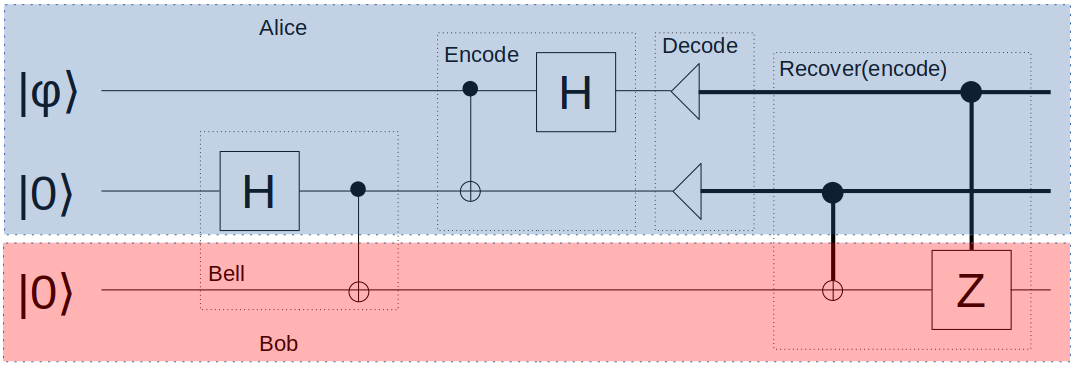
\includegraphics[width=1\textwidth]{tele_circuit.png}
            \caption{Quantum Teleportation Circuit}
            \label{fig:background-circuit-examplea}
          \end{minipage}
         %
          \begin{minipage}[b]{.50\textwidth}
                 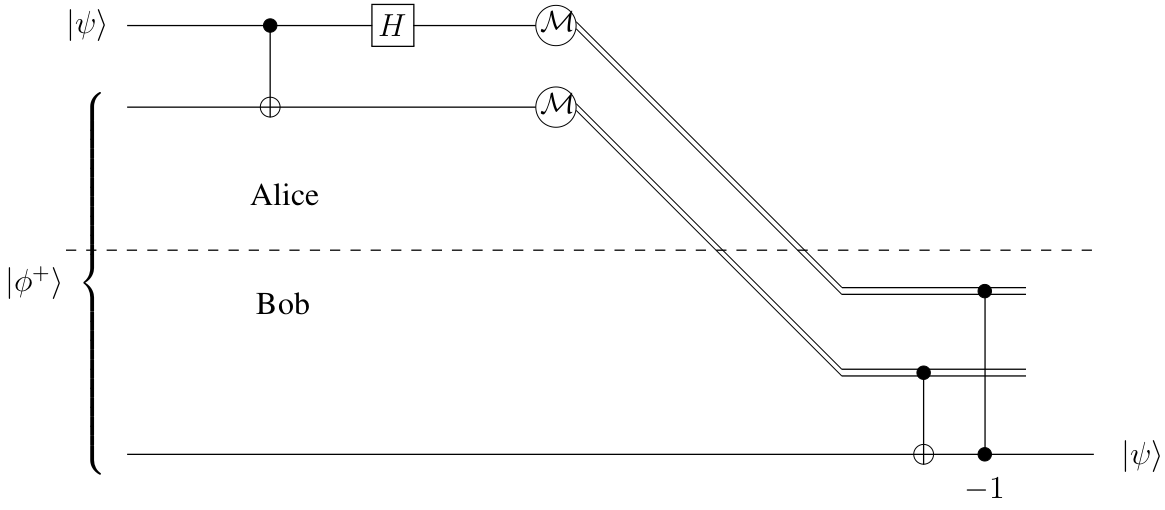
\includegraphics[width=1\textwidth]{teleportation.png}
            \caption{Quantum Teleportation Communication Diagram}
            \label{fig:background-circuit-exampleb}
          \end{minipage}
         }
  \label{fig:background-circuit-example}
\end{figure}

\noindent\textbf{\textit{Quantum Computations and Measurement.}} High-level quantum programming languages are usually designed to follow the \emph{QRAM model}~\cite{Knill1996}, where quantum computers are used as co-processors to classical computers. The classical computer generates descriptions of circuits to send to the quantum computer and then processes the measurement results.
Computation on a quantum value state consists of a series of \emph{quantum operations}, each of which acts on a subset of qubits in the value state. In the standard presentation, quantum computations are expressed as \emph{circuits}, as shown in \Cref{fig:background-circuit-examplea}, which constructs a circuit for quantum teleportation algorithm \cite{PhysRevLett.70.1895}, which sends a quantum message $\varphi$ from Alice to Bob, as shown in \Cref{fig:background-circuit-exampleb}.
In these circuits, each horizontal wire represents a qubit and boxes on these wires indicate quantum operations, or \emph{gates}. The circuit for $\texttt{bel1000}$ in \Cref{fig:background-circuit-examplea} uses two qubits and applies two gates: a \emph{Hadamard} (\coqe{H}) and \emph{controlled-not} (\coqe{CNOT}) gate to preprare a Bell pair above.
\ignore{
Applying a gate to a state \emph{evolves} the state. The traditional semantics of doing so is expressed by multiplying the state vector by the gate's corresponding matrix representation; single-qubit gates are 2-by-2 matrices, and two-qubit gates are 4-by-4 matrices. A gate's matrix must be \emph{unitary}, ensuring that it preserves the unitarity invariant of quantum states' amplitudes. An entire circuit can be expressed as a matrix by composing its constituent gates.
}

A \emph{measurement} operation extracts classical information from a quantum state, typically when a computation completes. Measurement collapses the state to a basis states with a probability related to the state's amplitudes. For example, measuring $\frac{1}{\sqrt{2}}(\ket{0} + \ket{1})$ in the computational basis will collapse the state to $\ket{0}$ with probability $\frac{1}{2}$ and likewise for $\ket{1}$, returning classical value 0 or 1, respectively. In all the programs discussed in this paper, we leave the final measurement operation implicit.

\noindent\textbf{\textit{Quantum Network based on Teleportation.}}
Almost all quantum network protocols are originated from the quantum teleportation algorithm \cite{PhysRevLett.70.1895}.
The circuit diagram in \Cref{fig:background-circuit-exampleb} describes a quantum teleportation circuit for communicating one qubit message between Alice and Bob.
In this algorithm, Alice sends a qubit message $\varphi$ to Bob via an entangled group $\phi^{+}$ consisting of two qubits.
Before sending the $\varphi$ qubit, Alice and Bob holds one qubit in the entangled qubit group $\phi^{+}$.
In the beginning, Alice entangles $\varphi$ with her holding $\phi^{+}$ qubit by using a CNOT gate following by a Hadamard gate.
Thus, after the two gate application, $\varphi$ joins the entangled group $\phi^{+}$.
Alice then measures her two holding qubits. This event produces two bits resulting from the measurement.
The measurement also has another conseuqnece since the three qubits are entangled;
that is, the remaining quantum information of the Alice's two qubits is pushed to store in Bob's remaining qubit.
Once Alice sends the two bits to Bob, he is able to reconstruct $\varphi$ through a proper treatment of his own qubit,
shown on the left of \Cref{fig:background-circuit-exampleb}.
In this paper, we will try to model the quantum teleportation concept
by abstracting away the details of the gates and measurement devices,
which represent a low-level circuit implementation of the quantum teleportation algorithm.

\liyi{Le: not very clear. need to add some pictures and explain in details how swaps work.}
\noindent\textbf{\textit{Extended Quantum Network Communication By Quantum Routing.}}
Quantum teleportation describes the circuit details of communicating quantum messages through two parties.
For a long distance communication, the quantum routing concept is involved.
A typical and near term possible technique to send quantum information through long distance is \textit{entanglement swap},
which relies on intermediate quantum repeaters between the two parties. Suppose Alice and Bob stay in two separate places and there is a quantum repeater, $r_1$ between them, they can create a long-distance entanglement in two steps. First, Alice and Bob each create an entanglement state with $r_1$; then $r_1$ performs a Bell state measurement locally. After measurement, the two original entanglements are destroyed and therefore, a new entanglement pair is created between Alice and Bob. 

Through the entanglement swaps, quantum messages can be sent through long-distance, with a consumption of qubit resources and reduction of success rate of transmitting the messages, because each entanglement pair destruction and creation requires qubit resources and has a certain percentage of failure. 
Since almost all quantum network protocols utilize the quantum teleportation and quantum routing as the guidance to send quantum messages, in QAM, we model quantum teleportation as the step to receive a message, and quantum routing as the step to transmit a message through a long distance by consuming some qubit resources and reducing some success rate.
% \liyi{later.}

\liyi{Le: need better description. Please help find the CHEM paper and modify. }
\noindent\textbf{\textit{Chemical Abstract Machine.}} Chemical abstract machine \cite{BERRY1992217} models multi-party communication behaviors as chemical reactions, where processes live in molecule cell structures and they can react by the reaction rules defining how molecule cells can connect together and processes living inside a cell can also communicate through the heating and cooling rules, 
defining the transformation between process active and inactive states, where active and inactive states represent processes being able to communicate or not.

% Writing a quantum algorithm now, with SQIR (but likewise with Quipper, Pyquil, Circ, etc.). Example: Shor’s
% Write quantum parts (QPE) 
% Classical parts via library functions in meta-language (Modular multiplier)
% Refer to particular quipper functions, e.g., for adding, subtraction, etc.
% https://www.mathstat.dal.ca/~selinger/quipper/doc/Quipper-Libraries-QFTAdd.html qft_add_in_place :: QDInt -> QDInt -> Circ (QDInt, QDInt), Add one QDInt onto a second, in place; i.e. (x,y) ↦ (x,x+y). Arguments are assumed to be of equal size. This implementation follows the implementation in Thomas G. Draper's paper "Addition on a Quantum Computer" which doesn't require the use of any ancilla qubits through a clever use of the quantum Fourier transform.
% Mention Q# too
% https://github.com/microsoft/QuantumLibraries/tree/main/Numerics/src
% Maybe Scaffold:
% Write oracles via “RKQC intrinsic” functions (see sec 4.1 of https://iopscience.iop.org/article/10.1088/2058-9565/ab8c2c/pdf). The intrinsics they talk about here are super simple (swap two registers or add two registers together)
% Quipper: Write in Haskell, build_circuit, is better
% Problems to solve: Efficient compilation, verification of that compilation
% Verification: Prior work with ReverC, but only classical gates
